\section{How to build a \gls{name}}

In the current incarnation of \glspl{name}, a documentation author writes a \gls{name} to adaptively describe relevant code programmers find while they browse the web.
A \gls{name} is an engine for generating explanations or demonstrations of code for a specific language or library, accessible as a simple web API.
When queried with the text of a web page, a \gls{name} detects instances of the language, parses them, and returns explanations for each one as formatted HTML that can be viewed in a tooltip.
These steps are decribed in detail below.

\begin{figure}
\centering
    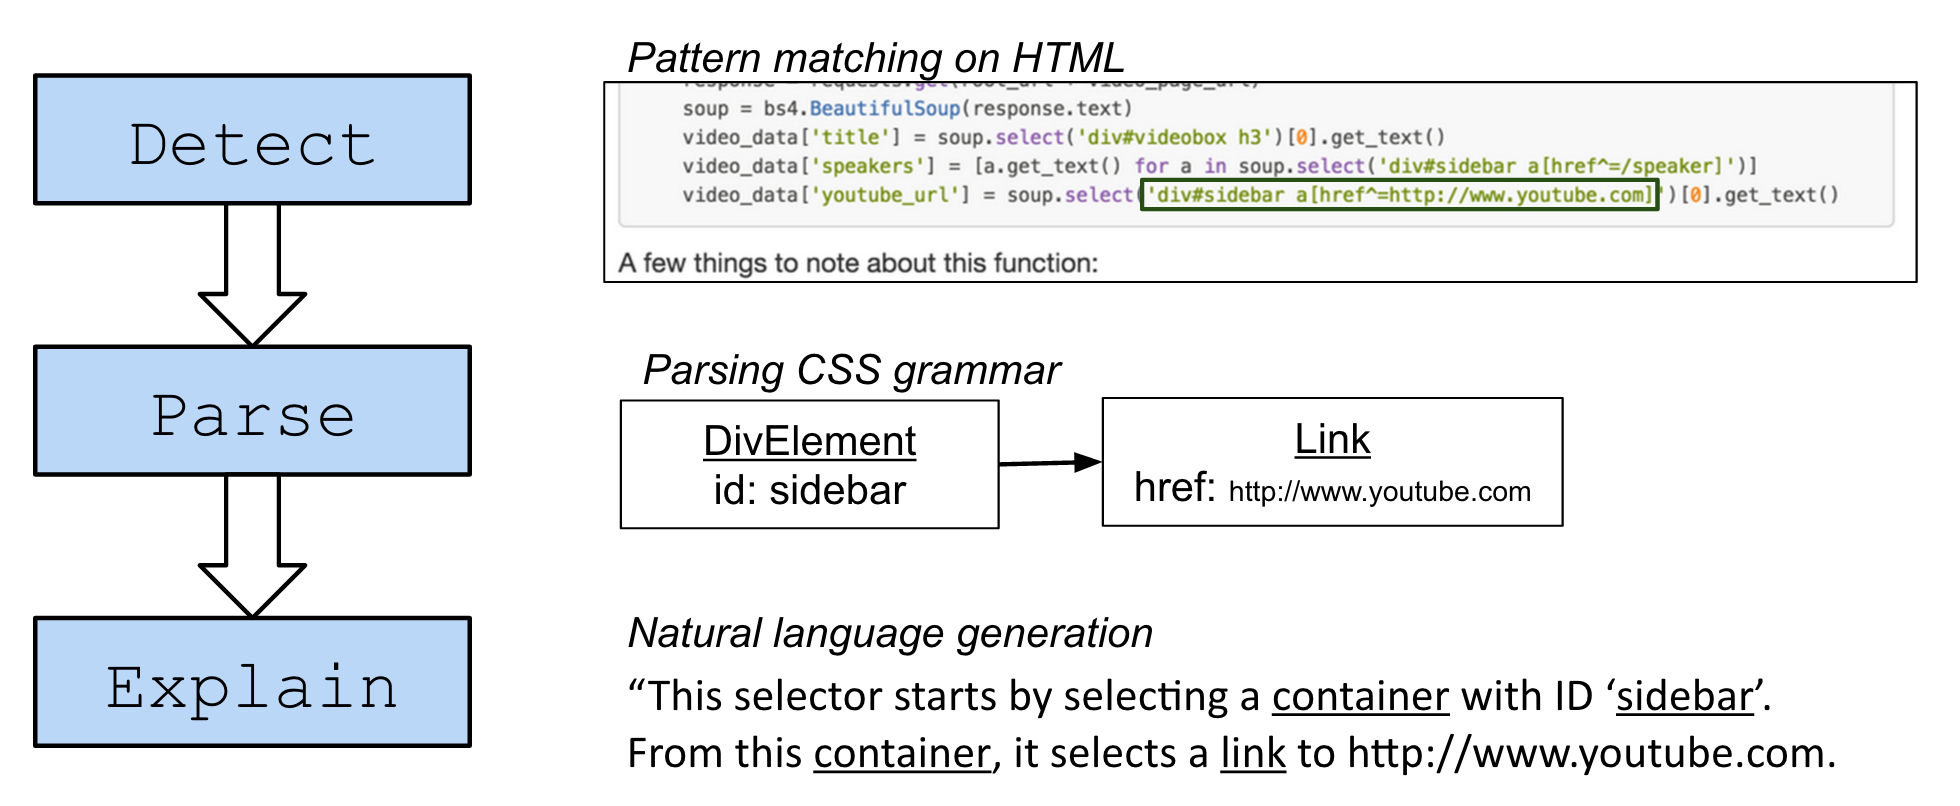
\includegraphics[width=.4\textwidth]{figures/explanation_pipeline}
    \caption{\Glspl{name} \emph{detect} relevant code snippets, \emph{parse} them, and then \emph{generate explanations}.  Here we show examples of the output of each stage of the pipeline for a \gls{name} that explains CSS selectors.}
    \label{fig:explanation_pipeline}
\end{figure}

By installing an addon for the browser, a programmer receives instant access to explanations from \gls{name} servers, which can be viewed as in-situ descriptions of code found while browsing (Figure~\ref{fig:browser_tutorons_markup}).
The addon queries existing \glspl{name} with the page source, receiving explanations of all instances of the language.
After receiving explanations, an explanation will appear in a tooltip overlaid on the document directly beneath the source any time the programmer selects an explainable string of text.

We call these explanations and demonstrations \emph{accelerators} given that they potentially increase the speed at which programmers can understand and make use of online code.
The \Glspl{name} addon can query many explanation servers for multi-language support within the same page.
In the future, we will allow users to switch off explanations for certain languages for which they do not want assistance.

The addon uses a \emph{push} method of fetching explanations rather than a \emph{pull} method --- it asks a server to detect all explainable instances of a language, instead of querying a server to attempt to explain the user's current selection.
This choice enables all explanations to be generated in a single batch when the user first accesses the page, reducing the load time to milliseconds instead of seconds to access explanations.
Furthermore, this resolves the problem where a user's selection may not cover a complete statement of the syntax of a language.
By pre-computing these explainable text regions, we can allow users to select explainable code with \emph{fuzzy boundaries} (see Figure~\ref{fig:fuzzy_boundaries}).

\begin{figure}
    \centering
    \framebox{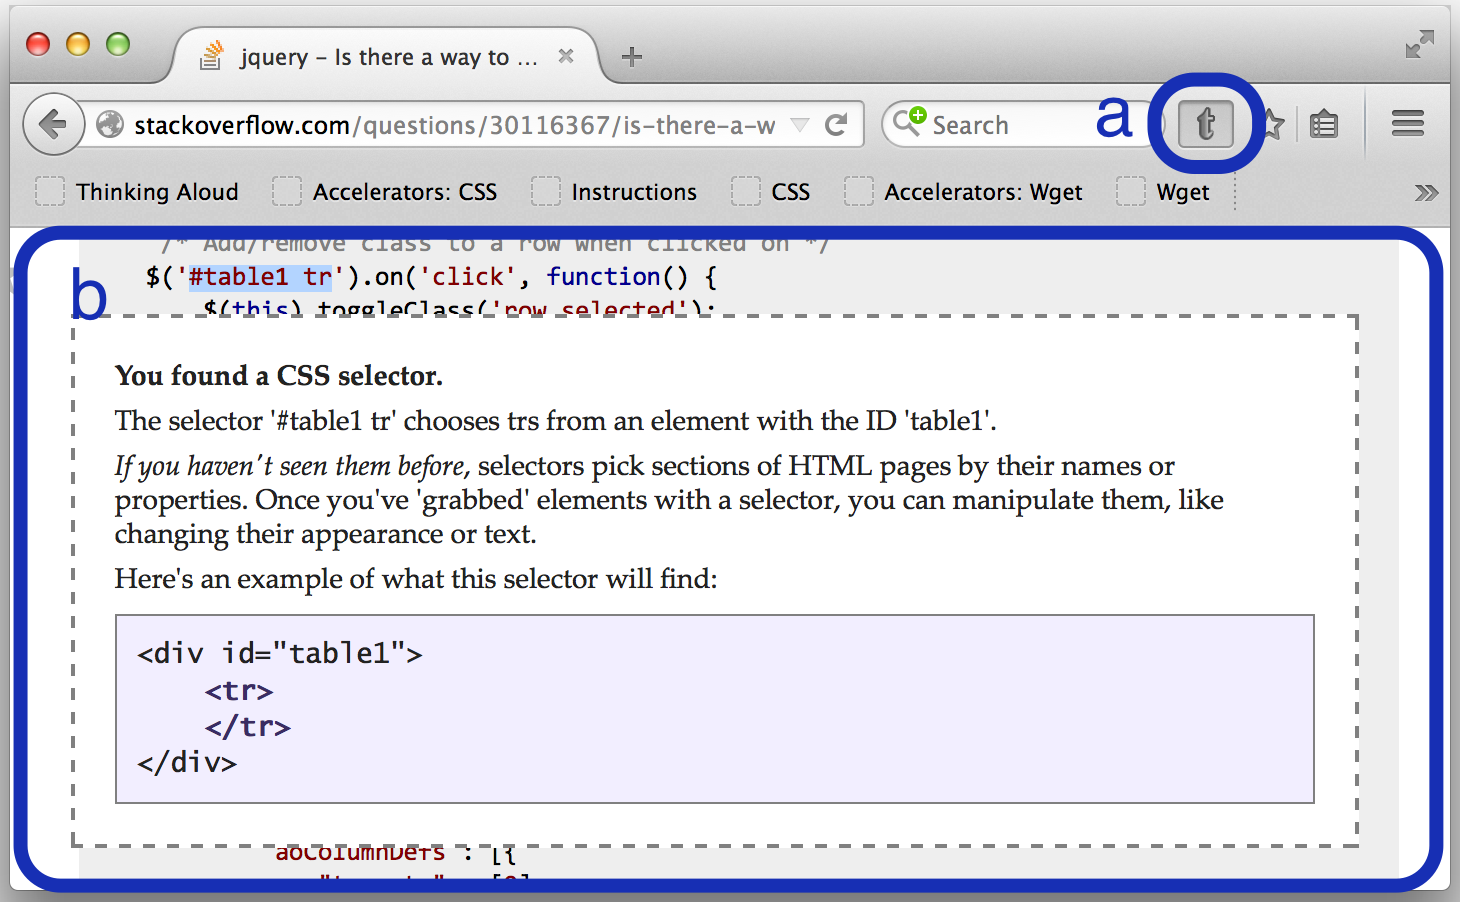
\includegraphics[width=.4\textwidth]{figures/browser_tutorons_markup}}
    \label{fig:browser_tutorons_markup}
    \caption{A user installs the \Glspl{name} addon.  \emph{(a)} Once she activates it, \emph{(b)} she can view automatically-generated, context-relevant explanations of code of supported languages in-situ while she browses programming help.}
\end{figure}

\begin{figure}
\centering{
    \subfigure[The CSS selector.]{
        \framebox{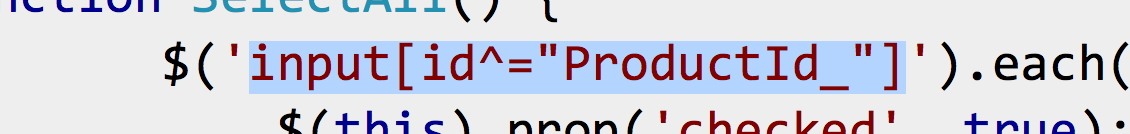
\includegraphics[width=.2\textwidth]{figures/selection_best}}
        \label{fig:selection_best}
    }
    \subfigure[The CSS selector with quotes.]{
        \framebox{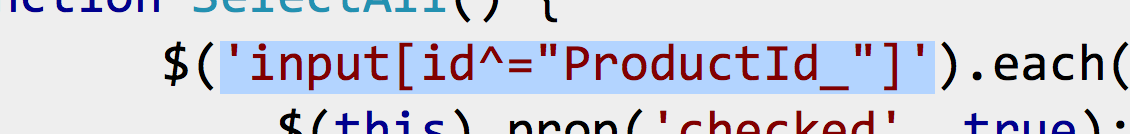
\includegraphics[width=.2\textwidth]{figures/selection_quotes}}
        \label{fig:selection_quotes}
    }
    \subfigure[A jQuery selection.]{
        \framebox{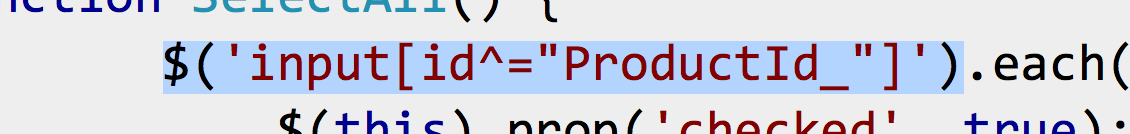
\includegraphics[width=.2\textwidth]{figures/selection_jquery}}
        \label{fig:selection_jquery}
    }
    \subfigure[A sloppy selection.]{
        \framebox{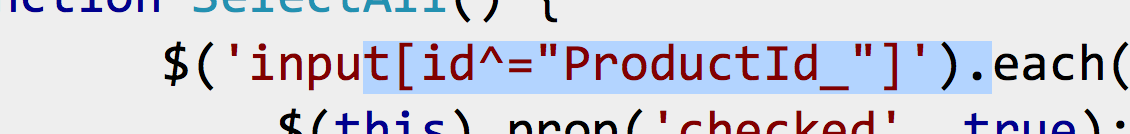
\includegraphics[width=.2\textwidth]{figures/selection_sloppy}}
        \label{fig:selection_sloppy}
    }
    \caption{
    The \Glspl{name} addon activates explanations for code when a user selects text.
    While explainable code fragments pre-computed on an explanation server, the addon enables users to view explanations with fuzzy selections.
    This lets them view hints without knowing the exact syntactic boundaries of the code they want to have described.
    }
    \label{fig:fuzzy_boundaries}
}
\end{figure}

In a world where \glspl{name} were prevalent and one or more existed for each language and library, what would prevent multiple \glspl{name} from explaining the same code?
We expect that in future versions, users can manage languages and libraries they want to explain from a central configuration interface.
Toolbars can be added to the browser to allow users to rapidly turn off explanations that they don't need.

A \gls{name} that resides on a server has to detect, parse and explain code.
We take some time to describe each of the steps in further detail here to offer an overview of strategies for finding relevant code in a page and generating useful explanations.

The \emph{detection} stage is tasked with extracting all code snippets that follow a language's grammar or a library's signatures from an HTML document.
In our own \gls{name} implementations, we reduce this to four steps.
First, we extract all blocks of code from HTML pages contained in a \texttt{<pre>} or multi-line \texttt{<code>} element on the page.
While not all online tutorials place code in these elements --- for instance, some post images of text files or nest it in a \texttt{<p>} or \texttt{<div>} --- we have found that a large number of tutorials and StackOverflow consistently formats code in this way.
Second, we extract all single lines or string symbols in each block of code, depending on the language we want to explain.
CSS selectors and regular expressions are often written as strings in larger Python or JavaScript programs, while command lines like wget contain a full line of code.
Third, candidate lines or strings are passed through a language-specific parser or pattern matcher to find which ones follow the grammar.
In an optional fourth step, the false positive detection rate can be reduced by filtering candidates to only those containing tokens highly representative of the language --- like searching for HTML tags in CSS selectors, or the \texttt{\textbackslash{}w}, \texttt{\textbackslash{}s}, or \texttt{\textbackslash{}d} symbols in regular expressions.

In the \emph{parsing} stage, detected code snippets are parsed into an intermediate representation
As programming languages necessarily have a parser, \gls{name} developers can use existing parsers as starting points.
We have found two method of building parsers to be helpful.
When supporting a frequently-used subset of a language, we recommend developing a lightweight parser using a parser generator like ANTLR\footnote{\url{www.antlr.org}}.
Then the \gls{name} author can create IR in format is simple to traverse when building explanations.
We found this workflow helpful when building an explainer of CSS selectors.
Alternately, when it is necessary to recognize a wide range of symbols and their semantics, \gls{name} authors should modify existing parsers, introducing hooks for extracting the IR.
For example, while writing a \gls{name} for \texttt{wget}, we avoided replicating complex command line parsing rules by modifying the source to simply parse the command line options and pipe these to a Python-based explanation script.

Finally, in the \emph{explanation} stage, IR is converted into natural language explanations.
The structure of generated language is highly dependent on domain.
For CSS selectors, it makes sense to perform pre-order tree traversal, describing selectors from descendant to ancestor.
Regular expressions can be described linearly, with branches at optional sub-patterns.
Command lines can be described by explaining each of the arguments, with special explanations generated for typical combinations of arguments like \texttt{--user} and \texttt{--password}.
As a \gls{name} generates HTML to be shown in a tooltip for each code snippet, it can optionally aesthetically emphasize key parts of the explanation.
